\subsection{Convolutional Neural Networks}
\label{back:cnn}

\acrfull{cnn}, a specialized type of feed-forward neural network, has become a cornerstone in \acrshort{dl} architectures. This architecture introduces a powerful approach to processing matrix data, especially images.
The foundations of \acrshort{cnn}s started all the way back in the 1960s, focusing on the visual cortex \cite{hubel1962receptive}, but they were first properly introduced to the \acrshort{ml} field in 1990 by Yan LeCun \cite{NIPS1989_53c3bce6}. Since then, \acrshort{cnn}s have undergone significant developments, leading to breakthroughs in various fields of artificial intelligence. \\
%
At their core, \acrshort{cnn}s rely on kernel operations, primarily convolutions, to calculate features. The two-dimensional convolution is a mathematical operation that can be formulated as follows:
\begin{equation}
   (f * g)(x, y) = \sum_{m=0}^{M-1} \sum_{n=0}^{N-1} f(m, n)g(x-m, y-n) 
\label{eq:conv}
\end{equation}
Here $f$ is the kernel, $g$ is the input matrix, $x$ and $y$ are the row and column of the input matrix, $m$ and $n$ are the row and column in the kernel, and $M$ and $N$ are the number of rows and columns in $g$ respectively. This is further illustrated in Figure \ref{fig:2dconv}.
%
\begin{figure}[!h]
    \centering
    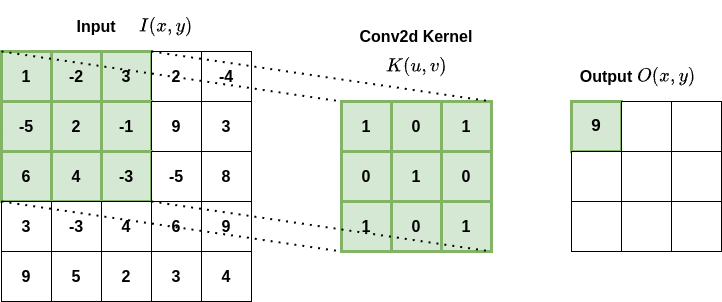
\includegraphics[width=0.8\linewidth]{figures/convolution.png}
    \caption{2D Convolutional operation example. The dot product between the kernel $K$ and each submatrix of input $I$ is computed and added to output $O$. This specific convolution reduces dimensionality.}
    \label{fig:2dconv}
\end{figure}
\clearpage
 When performing cross-correlation convolution, only the size of the kernel is used to store neurons, compared to linear layers, where all the weights between layers need to be stored. This dramatically reduces the memory requirements compared to \acrshort{fcnn}s. The convolutional operation is essentially multiple matrix multiplication between different regions in the data and a kernel. These multiplications can be performed in a parallelized manner. Matrix multiplications have undergone significant improvement over the years \cite{karstadt2020matrix}, and have, with the introduction of CUDA, been further optimized for better-suited hardware architectures such as \acrshort{gpu}s. With the rapid improvements of \acrshort{gpu}s \cite{bell2008efficient}, the computational efficiency of both linear and convolutional layers has improved drastically. This has resulted in overall lower energy requirements for model training, reduced training times, and the introduction of distributed large-scale model training \cite{mungoli2023scalable}. 

Unlike fully connected layers that compute global interactions, convolution operations in \acrshort{cnn}s focus on local regions of data as seen in Figure \ref{fig:2dconv}. This approach allows for improved feature extraction, making them particularly effective for tasks involving spatial data, compared to \acrshort{fcnn}s. 

Furthermore, due to \acrshort{cnn}s inherent quality of feature extraction, they are not as prone to the vanishing gradient problem \cite{tan2019vanishing} as \acrshort{fcnn}s. This occurs when gradients propagated backward through the layers become very small, making it difficult for the network to update its weights effectively. \\

\begin{figure}[!h]
    \centering
    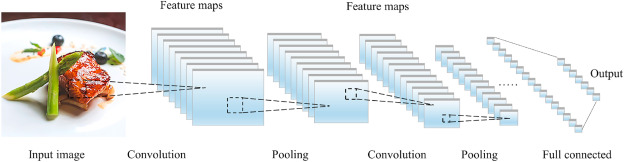
\includegraphics[scale=0.8]{figures/conv2d.jpg}
    \caption{Example of a \acrshort{cnn} by Liu et al. \cite{LIU2021193}}
    \label{fig:cnn}
\end{figure}

\subsubsection{Pooling}
%
In \acrshort{cnn}s, a convolutional layer is followed by an activation function $f$ and then a pooling operation as seen in Figure \ref{fig:2dconv}. Pooling reduces the spatial dimensions of the data, making the network more computationally efficient and helping to extract more dominant features \cite{SUN201796}.
The three most common pooling operations are max pooling, min pooling, and average pooling, with max pooling being the most widely used. Max pooling works by selecting the maximum value from a defined region of the input feature map.
\begin{figure}[!h]
\centering
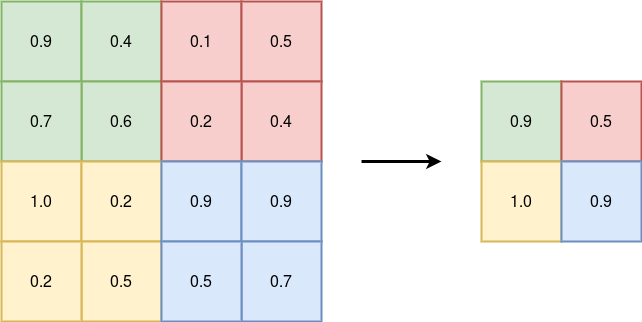
\includegraphics[scale=0.4]{figures/pooling.png}
\caption{Example of a $2 \times 2$ max pooling operation with stride 2}
\label{fig:maxpool}
\end{figure}
Figure \ref{fig:maxpool} illustrates a $2 \times 2$ max pooling operation with a stride of 2. The pooling kernel moves across the input matrix $M$, selecting the maximum value from each $2 \times 2$ region it covers. This process is repeated until the entire input has been processed, resulting in reduced spatial dimensions in both height and width. 